\section{Results}

Voici des examples des cartes d'équilibres que je peux générer avec l'outil. Tout les résultats sont générés pour un cas de panne moteur(s) au décollage en concervant un angle de montée de 2°. (Les conditions seront résumés dans un tableau pour la version final)

Mon idée est de faire passer le plus d'information avec le moins de graphs possible. Je me concentrerai sur la phase de décollage avec des cartes en vitesse-versus-dérapage. En plus j'ajouterai un example de répartition de poussée et d'attitude de l'avion typique pour une DEP avec panne moteur. Qu'est-ce que vous en penser?

\begin{figure}[hbt!]
	\centering
	\begin{subfigure}{0.49\textwidth}
		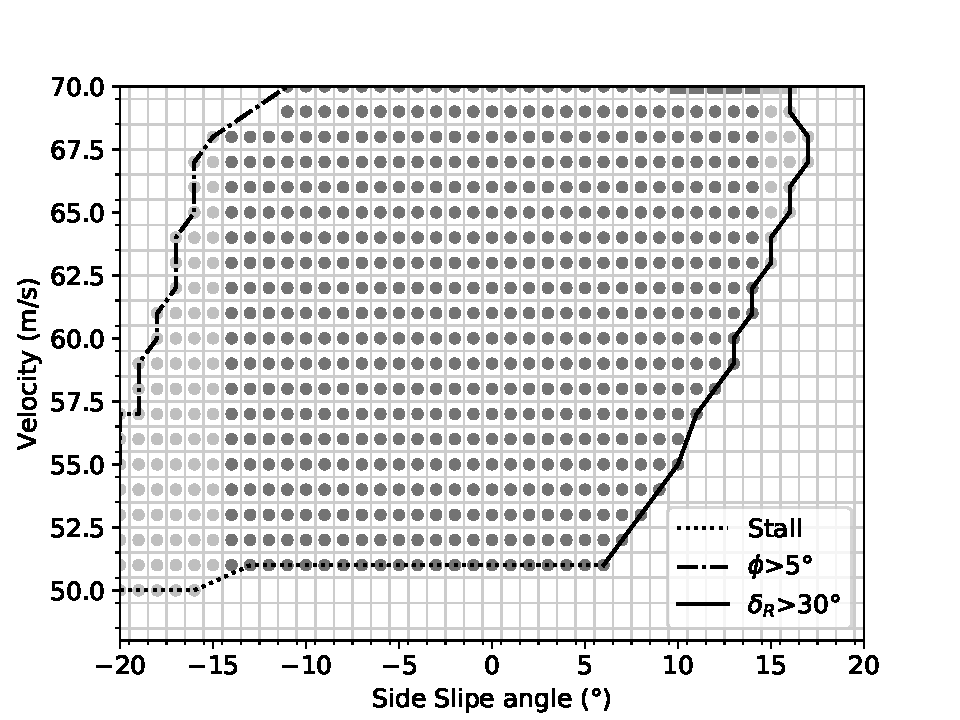
\includegraphics[width=0.95\textwidth]{originalMapBetaVelfin1Eng3RudFalse}
		\caption{Original ATR72 with one engine failure.}
		\label{fig:originalfin1_3engine}
	\end{subfigure}
	\begin{subfigure}{0.49\textwidth}
		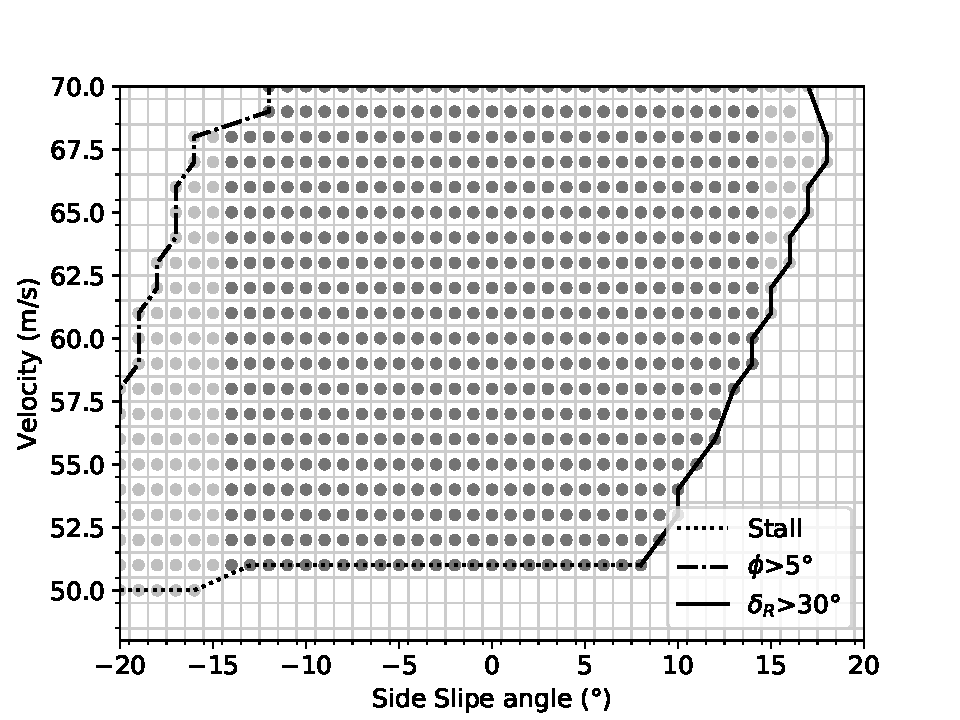
\includegraphics[width=0.95\textwidth]{originalMapBetaVelfin1Eng15RudFalse}
		\caption{ATR with 12 engines, three inoperatives.}
		\label{fig:originalfin1_15engine}
	\end{subfigure}
	\caption{Original ATR with \ref{fig:originalfin1_3engine} twin engine, one inoperational and \ref{fig:originalfin1_15engine} twelve engines, three inoperationals. Only the rudder is used to compensate the yawing moment.}
\end{figure}

\begin{figure}
	\begin{subfigure}{0.49\textwidth}
		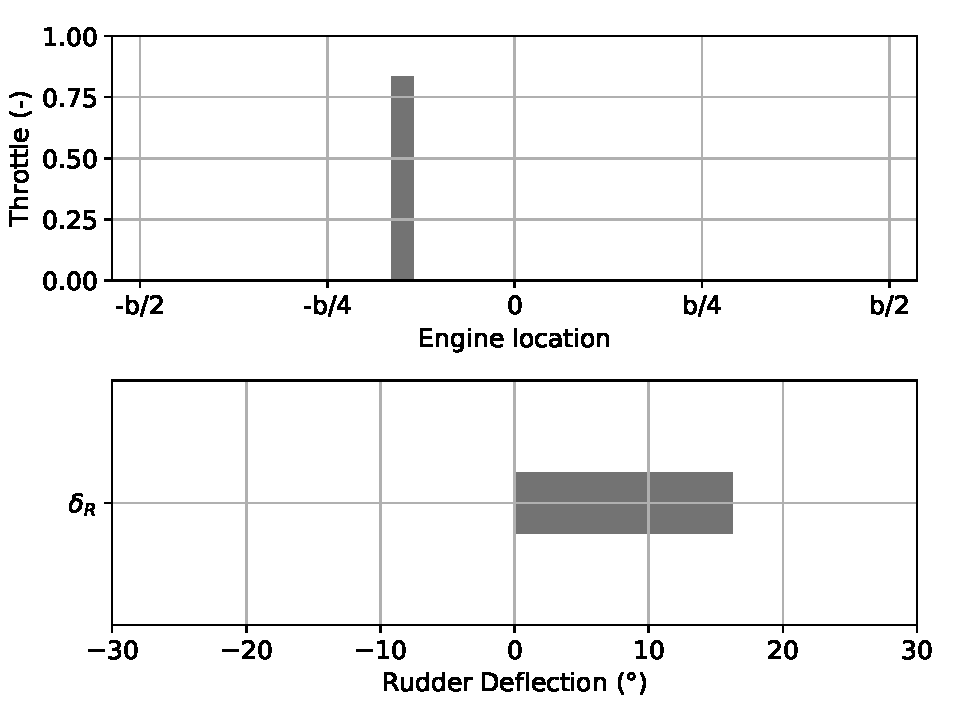
\includegraphics[width=0.95\textwidth]{Defloriginalfin1Eng3RudFalse}
		\caption{Original ATR72 with one engine failure.}
		\label{fig:Defloriginalfin1_3engine}
	\end{subfigure}
	\begin{subfigure}{0.49\textwidth}
		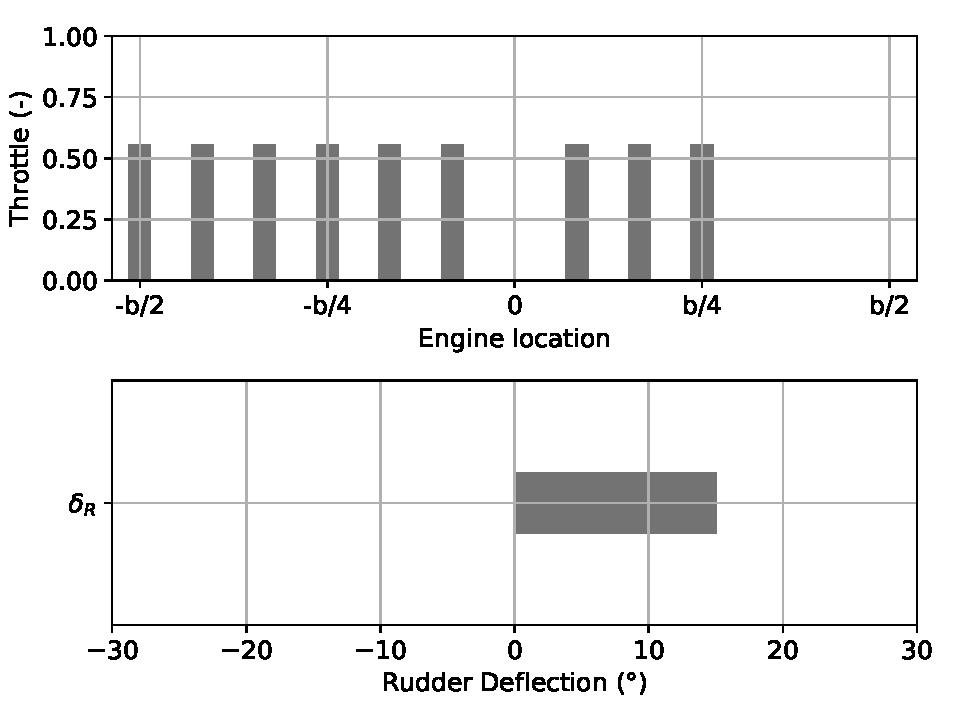
\includegraphics[width=0.95\textwidth]{Defloriginalfin1Eng15RudFalse}
		\caption{Original ATR with twelve engines, three inoperatives.}
		\label{fig:Defloriginalfin1_15engine}
	\end{subfigure}
	\caption{Throttle level and rudder deflection for trim at V=60m/s, $\beta=0$}
\end{figure}

\begin{figure}[hbt!]
		\centering
		\begin{subfigure}{0.49\textwidth}
			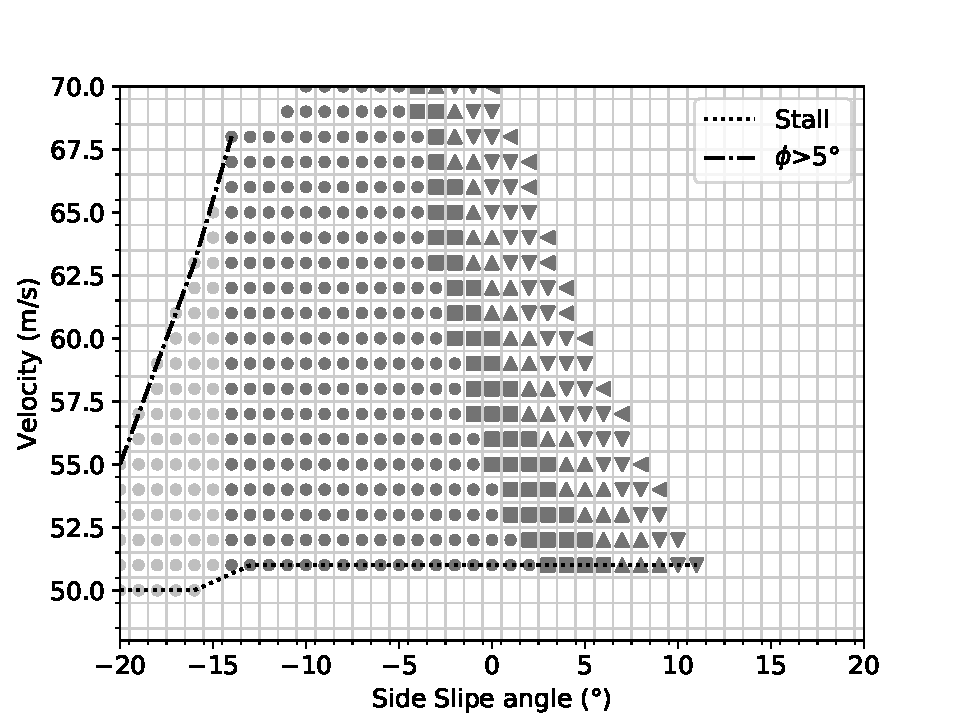
\includegraphics[width=0.95\textwidth]{DEPoriginalMapBetaVelfin1Eng15RudTrue}
			\caption{Flight envelop, ATR with 12 engines, three inoperatives.}
			\label{fig:DEPoriginalfin1_15engine}
		\end{subfigure}
		\begin{subfigure}{0.49\textwidth}
			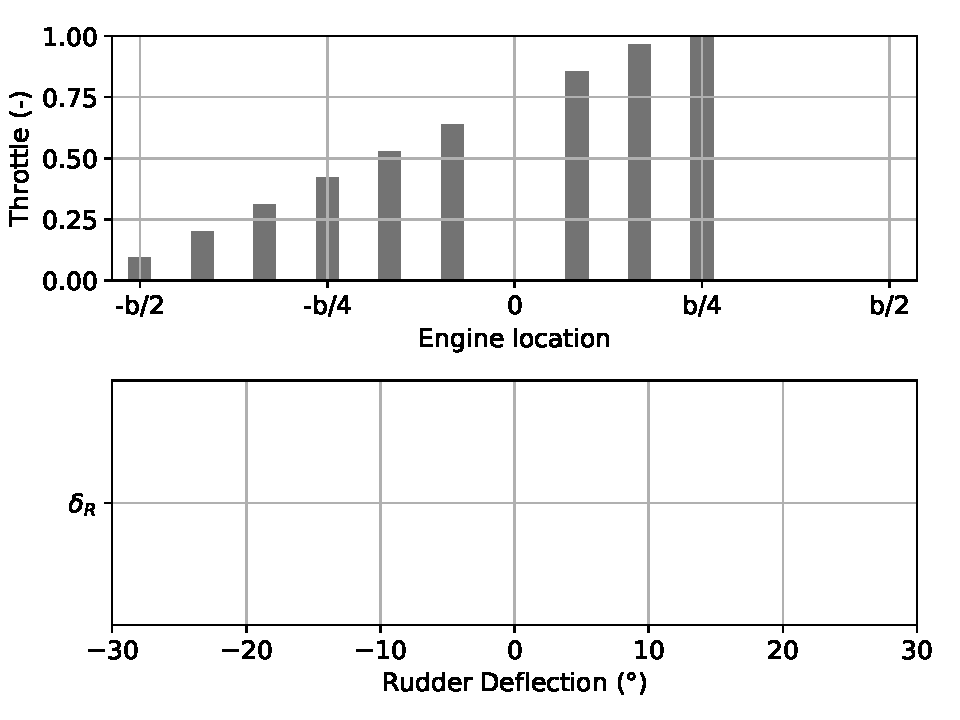
\includegraphics[width=0.95\textwidth]{DeflDEPoriginalfin1Eng15RudTrue}
			\caption{Throttle level and Rudder deflection at 60m/s and $\beta=0\degree$, ATR72 with 12 engines, three inoperatives.}
			\label{fig:DeflDEPoriginalfin1_15Eng}
		\end{subfigure}
		\caption{ATR72 using only differential thrust. Circles indicate an equilibrium point, rectangle indicate an equilibrium with at least one engine at saturation (full throttle)}
\end{figure}

\begin{figure}[hbt!]
	\centering
	\begin{subfigure}{0.49\textwidth}
		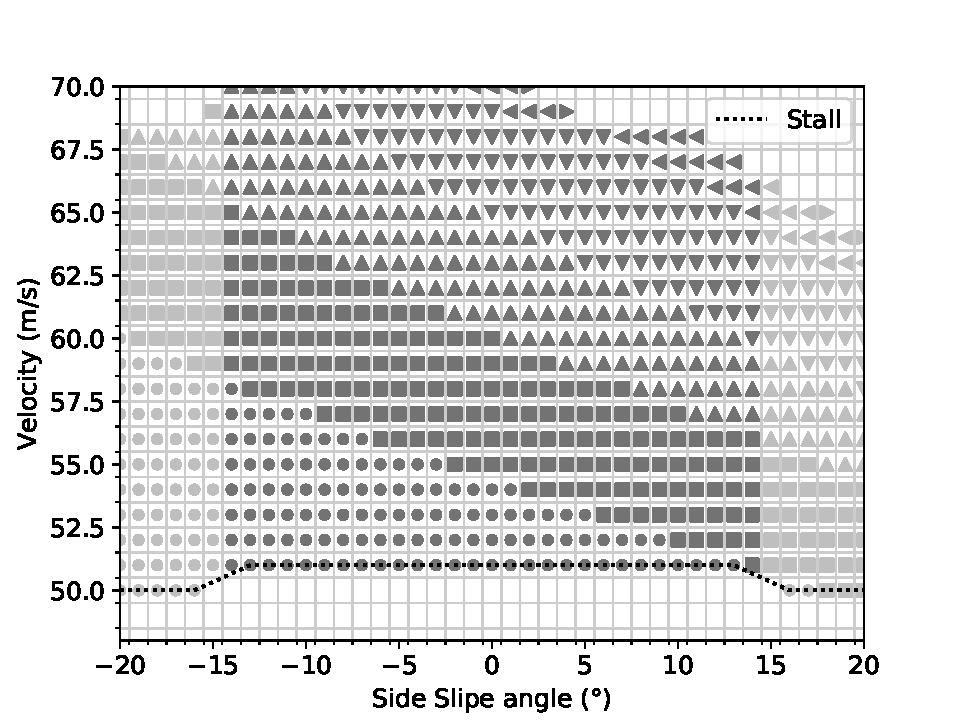
\includegraphics[width=0.95\textwidth]{DEPoriginalMapBetaVelfin07Eng15RudTrue}
		\caption{ATR with 12 engines, three inoperatives and $S_v=0.7S_{v_0}$. Rudder not used. Circles indicate an equilibrium point, rectangle indicate an equilibrium with at least one engine at saturation (full throttle)}
		\label{fig:DEPoriginalfin07_15engine}
	\end{subfigure}
	\begin{subfigure}{0.49\textwidth}
		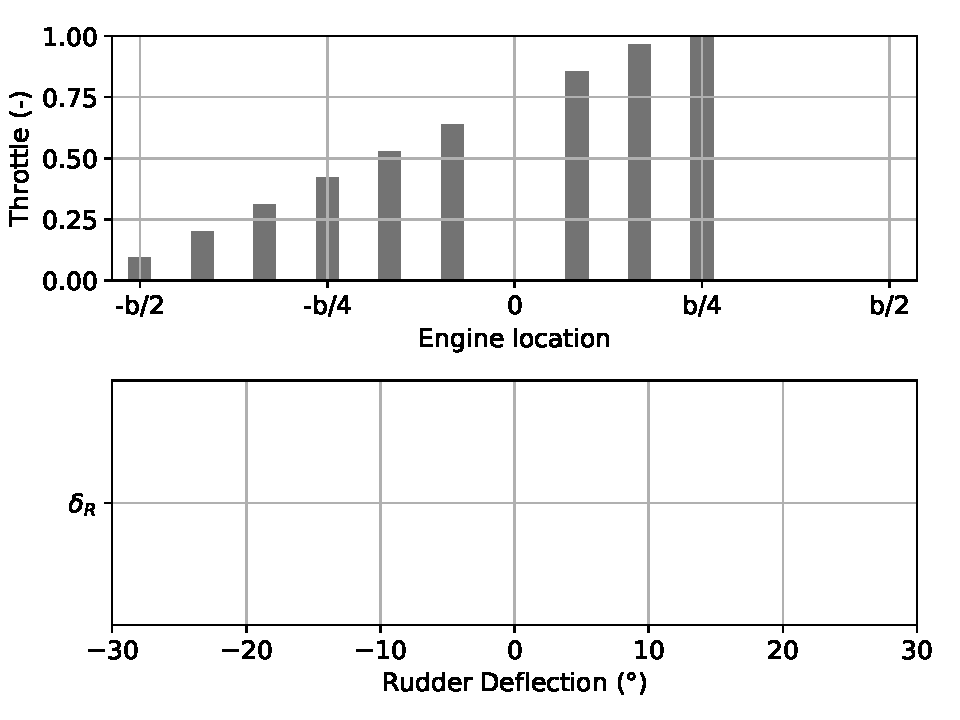
\includegraphics[width=0.95\textwidth]{DeflDEPoriginalfin07Eng15RudTrue}
		\caption{Throttle level and Rudder deflection at 60m/s and $\beta=0\degree$, ATR72 with 12 engines, three inoperatives, $S_v=0.7S_{v_0}$.}
		\label{fig:DeflDEPoriginalfin07_15Eng}
	\end{subfigure}
\end{figure}

%----- Study Case -----
%One original ATR72 at take off without failed engine next to the same ATR72 at Take off with SEF:
%	Shows that Vmc is found for take off,
%	Show that control is maintained at 1.3Vsr (=15° yaw toward inoperative engine)
%	shows that no equilibrium exists,
%	eventually show the degradation of equilibrium with reduced VT
%	Show the engine saturation at high speed

%Show the same ATR with distributed propulsion:
%	Show input histogramme with and without rudder
%	Show map without rudder and with small rudder
%	Show map with small fin and rudder
%
%At take off means :
%	3% slope for more than 4 engine condition, 
%	2.4 % for twin engine with landing gear retracted (CS.25.121)
%	Not necessarly full power but explore by going higher (in speed mostly)
%	0 altitude
%Maybe replace velocity scale by Vsr, 1.3Vsr etc... as defined by CS

% ATR at 21.5T Vapp=56m/s if it is 1.13Vsr then Vsr=49.55m/s, 1.3Vsr=64.4m/s
% Eventually look at the 20° turns requirement from the certif

%
%Determine 1.3V_{sr} for CS25.147 stating 15° yaw in the direction of the inoperative engine.
%STATE MINIMUM DRAG and 